\section{Accessing hardware devices}

\subsection{Describing non-discoverable hardware: Device Tree}

\begin{frame}{Describing non-discoverable hardware}
  \begin{columns}
    \column{0.3\textwidth}
    \begin{enumerate}
    \item<1> Directly in the {\bf OS/bootloader code}
    \item<2> Using {\bf ACPI} tables
    \item<3> Using a {\bf Device Tree}
    \end{enumerate}
    \column{0.7\textwidth}
    \only<1> {
      \begin{itemize}
      \item Using compiled data structures, typically in C
      \item How it was done on most embedded platforms in Linux, U-Boot.
      \item Considered not maintainable/sustainable on ARM32, which
        motivated the move to another solution.
      \end{itemize}
    }
    \only<2> {
      \begin{itemize}
      \item On {\em x86} systems, but also on a subset of ARM64 platforms
      \item Tables provided by the firmware
      \end{itemize}
    }
    \only<3> {
      \begin{itemize}
      \item Originates from {\bf OpenFirmware}, defined by Sun, used on
        SPARC and PowerPC
        \begin{itemize}
        \item That's why many Linux/U-Boot functions related to DT have
          a \code{of_} prefix
        \end{itemize}
      \item Now used by most embedded-oriented CPU architectures that run
        Linux: ARC, ARM64, RISC-V, ARM32, PowerPC, Xtensa, MIPS, etc.
      \item Writing/tweaking a DT is necessary when porting Linux to a
        new board, or when connecting additional peripherals
      \end{itemize}
    }
  \end{columns}
\end{frame}

\begin{frame}{Device Tree: from source to blob}
  \begin{columns}
    \column{0.7\textwidth}
    \begin{itemize}
    \item A tree data structure describing the hardware is written by a
      developer in a {\bf Device Tree Source} file, \code{.dts}
    \item Processed by the {\bf Device Tree Compiler}, \code{dtc}
    \item Produces a more efficient representation: {\bf Device Tree
        Blob}, \code{.dtb}
    \item Additional C preprocessor pass
    \item \code{.dtb} $\rightarrow$ accurately describes the hardware platform in an {\bf OS-agnostic} way.
    \item \code{.dtb} $\approx$ few dozens of kilobytes
    \item DTB also called {\bf FDT}, {\em Flattened Device Tree}, once
      loaded into memory.
      \begin{itemize}
      \item \code{fdt} command in U-Boot
      \item \code{fdt_} APIs
      \end{itemize}
    \end{itemize}
    \column{0.3\textwidth}
    \includegraphics[height=0.7\textheight]{slides/sysdev-hw-devices/dts-to-dtb.pdf}
  \end{columns}
\end{frame}

\begin{frame}[fragile]{dtc example}
  \footnotesize
  \begin{columns}[t]
    \column{0.5\textwidth}
    \begin{block}{}
\begin{verbatim}
$ cat foo.dts
/dts-v1/;

/ {
        welcome = <0xBADCAFE>;
        bootlin {
                webinar = "great";
                demo = <1>, <2>, <3>;
        };
};
\end{verbatim}
    \end{block}
    \pause
    \begin{block}{}
\begin{verbatim}
$ dtc -I dts -O dtb -o foo.dtb foo.dts
$ ls -l foo.dt*
-rw-r--r-- 1 thomas thomas 169 ... foo.dtb
-rw-r--r-- 1 thomas thomas 102 ... foo.dts
\end{verbatim}
    \end{block}
    \pause
    \column{0.5\textwidth}
    \begin{block}{}
\begin{verbatim}
$ dtc -I dtb -O dts foo.dtb
/dts-v1/;

/ {
        welcome = <0xbadcafe>;

        bootlin {
                webinar = "great";
                demo = <0x01 0x02 0x03>;
        };
};
\end{verbatim}
    \end{block}
  \end{columns}
\end{frame}

\begin{frame}{Where are Device Tree Sources located ?}
  \begin{itemize}
  \item Even though they are OS-agnostic, {\bf no central and
      OS-neutral} place to host Device Tree sources and share them
    between projects
    \begin{itemize}
    \item Often discussed, never done
    \end{itemize}
  \item In practice, the Linux kernel sources can be considered as the
    {\bf canonical location} for Device Tree Source files
    \begin{itemize}
    \item \code{arch/<ARCH>/boot/dts}
    \item $\approx$ 4500 Device Tree Source files (\code{.dts} and
          \code{.dtsi}) in Linux as of 6.0.
    \end{itemize}
  \item Duplicated/synced in various projects
    \begin{itemize}
    \item U-Boot, Barebox, TF-A
    \end{itemize}
  \end{itemize}
\end{frame}

\begin{frame}{Device Tree base syntax}
  \begin{columns}
    \column{0.5\textwidth}
    \begin{itemize}
    \item Tree of {\bf nodes}
    \item Nodes with {\bf properties}
    \item Node $\approx$ a device or IP block
    \item Properties $\approx$ device characteristics
    \item Notion of {\bf cells} in property values
    \item Notion of {\bf phandle} to point to other nodes
    \item \code{dtc} only does syntax checking, no semantic validation
    \end{itemize}
    \column{0.5\textwidth}
    \begin{center}
      \includegraphics[height=0.6\textheight]{slides/sysdev-hw-devices/dt-basic-syntax.pdf}
    \end{center}
  \end{columns}
\end{frame}

\begin{frame}[fragile]{DT overall structure: simplified example}
  \begin{columns}
    \column{0.6\textwidth}
    \begin{onlyenv}<1>
      \begin{block}{}
\begin{minted}[fontsize=\tiny]{perl}
/ {
  #address-cells = <1>;
  #size-cells = <1>;
  model = "TI AM335x BeagleBone Black";
  compatible = "ti,am335x-bone-black", "ti,am335x-bone", "ti,am33xx";

  cpus { ... };
  memory@80000000 { ... };
  chosen { ... };
  ocp {
    intc: interrupt-controller@48200000 { ... };
    l4_wkup: interconnect@44c00000 {
      usb0: usb@47401300 { ... };
      i2c0: i2c@40012000 { ... };
    };
  };
};
\end{minted}
      \end{block}
    \end{onlyenv}
    \begin{onlyenv}<2>
      \begin{block}{}
\begin{minted}[fontsize=\tiny]{perl}
/ {
  cpus {
    #address-cells = <1>;
    #size-cells = <0>;
    cpu0: cpu@0 {
      compatible = "arm,cortex-a8";
      enable-method = "ti,am3352";
      device_type = "cpu";
      reg = <0>;
    };
  };

  memory@0x80000000 {
    device_type = "memory";
    reg = <0x80000000 0x10000000>; /* 256 MB */
  };

  chosen {
    bootargs = "";
    stdout-path = &uart0;
  };

  ocp { ... };
};
\end{minted}
      \end{block}
    \end{onlyenv}
    \begin{onlyenv}<3>
      \begin{block}{}
\begin{minted}[fontsize=\tiny]{perl}
/ {
  cpus { ... };
  memory@0x80000000 { ... };
  chosen { ... };

  ocp {
    compatible = "simple-pm-bus";
    clocks = <&l3_clkctrl AM3_L3_L3_MAIN_CLKCTRL 0>;
    clock-names = "fck";
    #address-cells = <1>;
    #size-cells = <1>;

    intc: interrupt-controller@48200000 { ... };

    l4_wkup: interconnect@44c00000 {
      compatible = "ti,am33xx-l4-wkup", "simple-pm-bus";
      reg = <0x44c00000 0x800>, <0x44c00800 0x800>,
            <0x44c01000 0x400>, <0x44c01400 0x400>;
      reg-names = "ap", "la", "ia0", "ia1";
      #address-cells = <1>;
      #size-cells = <1>;

      usb0: usb@47401300 { ... };
      i2c0: i2c@40012000 { ... };
    };
  };
};
\end{minted}
      \end{block}
    \end{onlyenv}
    \begin{onlyenv}<4>
      \begin{block}{}
\begin{minted}[fontsize=\tiny]{perl}
/ {
  cpus { ... };
  memory@0x80000000 { ... };
  chosen { ... };
  ocp {

    intc: interrupt-controller@48200000 {
      compatible = "ti,am33xx-intc";
      interrupt-controller;
      #interrupt-cells = <1>;
      reg = <0x48200000 0x1000>;
    };

    l4_wkup: interconnect@44c00000 {

      usb0: usb@47401300 {
        compatible = "ti,musb-am33xx";
        reg = <0x1400 0x400>, <0x1000 0x200>;
        reg-names = "mc", "control";
        interrupts = <18>;
        dr_mode = "otg";
        dmas = <&cppi41dma  0 0 &cppi41dma  1 0 ...>;
        status = "okay";
      };

      i2c0: i2c@40012000 { ... };
    };
  };
};
\end{minted}
      \end{block}
    \end{onlyenv}
    \begin{onlyenv}<5>
      \begin{block}{}
\begin{minted}[fontsize=\tiny]{perl}
/ {
  cpus { ... };
  memory@0x80000000 { ... };
  chosen { ... };
  ocp {
    intc: interrupt-controller@48200000 { ... };
    l4_wkup: interconnect@44c00000 {
      usb0: usb@47401300 { ... };

      i2c0: i2c@40012000 {
        compatible = "ti,omap4-i2c";
        #address-cells = <1>;
        #size-cells = <0>;
        reg = <0x0 0x1000>;
        interrupts = <70>;
        status = "okay";
        pinctrl-names = "default";
        pinctrl-0 = <&i2c0_pins>;
        clock-frequency = <400000>;

        baseboard_eeprom: baseboard_eeprom@50 {
          compatible = "atmel,24c256";
          reg = <0x50>;
        };
      };
    };
  };
};
\end{minted}
      \end{block}
    \end{onlyenv}
    \column{0.4\textwidth}
    \includegraphics[width=\textwidth]{slides/kernel-hw-devices/simple-hardware.pdf}
  \end{columns}
\end{frame}

\begin{frame}[fragile]{Device Tree inheritance}
  \begin{itemize}
  \item Device Tree files are not monolithic, they can be split in
    several files, including each other.
  \item \code{.dtsi} files are included files, while \code{.dts} files
    are {\em final} Device Trees
    \begin{itemize}
    \item Only \code{.dts} files are accepted as input to \code{dtc}
    \end{itemize}
  \item Typically, \code{.dtsi} will contain
    \begin{itemize}
    \item definitions of SoC-level information
    \item definitions common to several boards
    \end{itemize}
  \item The \code{.dts} file contains the board-level information
  \item The inclusion works by {\bf overlaying} the tree of the
    including file over the tree of the included file.
  \item Allows an including file to {\bf override} values specified by
    an included file
  \item Uses the C pre-processor \code{#include} directive
  \end{itemize}
\end{frame}

\begin{frame}{Device Tree inheritance example}
  \begin{center}
    \includegraphics[width=\textwidth]{slides/kernel-hw-devices/dt-inheritance.pdf}
  \end{center}
\end{frame}

\begin{frame}[fragile]{Inheritance and labels}

  \begin{columns}[t]
    \column{0.5\textwidth}
    Doing:
    \begin{block}{soc.dtsi}
      {\tiny
\begin{minted}{perl}
/ {
  ocp {
    uart0: serial@0 {
      compatible = "ti,am3352-uart", "ti,omap3-uart";
      reg = <0x0 0x1000>;
      status = "disabled";
    };
  };
};
\end{minted}
      }
    \end{block}

    \begin{block}{board.dts}
      {\tiny
\begin{minted}{perl}
#include "soc.dtsi"

/ {
  ocp {
    serial@0 {
      status = "okay";
    };
  };
};
\end{minted}
      }
    \end{block}

    \column{0.5\textwidth}
    \begin{onlyenv}<2>
    Is exactly equivalent to:

    \begin{block}{soc.dtsi}
      {\tiny
\begin{minted}{perl}
/ {
  ocp {
    uart0: serial@0 {
      compatible = "ti,am3352-uart", "ti,omap3-uart";
      reg = <0x0 0x1000>;
      status = "okay";
    };
  };
};
\end{minted}
      }
    \end{block}

    \begin{block}{board.dts}
      {\tiny
\begin{minted}{perl}
#include "soc.dtsi"

&uart0 {
  status = "okay";
};
\end{minted}
        }
      \end{block}

      $\rightarrow$ this solution is now often preferred
      \end{onlyenv}
  \end{columns}

\end{frame}

\begin{frame}{DT inheritance in Bone Black support}
  \begin{center}
    \includegraphics[height=0.8\textheight]{slides/kernel-hw-devices/dt-inheritance-bbb.pdf}
  \end{center}
\end{frame}

\begin{frame}{Device Tree design principles}
  \begin{itemize}
  \item {\bf Describe hardware} (how the hardware is), not
    configuration (how I choose to use the hardware)
  \item {\bf OS-agnostic}
    \begin{itemize}
    \item For a given piece of HW, Device Tree should be the same for
      U-Boot, FreeBSD or Linux
    \item There should be no need to change the Device Tree when updating the OS
    \end{itemize}
  \item Describe {\bf integration of hardware components}, not the internals
    of hardware components
    \begin{itemize}
    \item The details of how a specific device/IP block is working is
      handled by code in device drivers
    \item The Device Tree describes how the device/IP block is
      connected/integrated with the rest of the system: IRQ lines, DMA
      channels, clocks, reset lines, etc.
    \end{itemize}
  \item Like all beautiful design principles, these principles are
    sometimes violated.
  \end{itemize}
\end{frame}

\begin{frame}{Device Tree specifications}
  \begin{columns}
    \column{0.7\textwidth}
    \begin{itemize}
    \item How to write the correct nodes/properties to describe a
      given hardware platform~?
    \item {\bf DeviceTree Specifications} $\rightarrow$ base Device
      Tree syntax + number of standard properties.
      \begin{itemize}
      \item \url{https://www.devicetree.org/specifications/}
      \item Not sufficient to describe the wide variety of hardware.
      \end{itemize}
    \item {\bf Device Tree Bindings} $\rightarrow$ documents that each
      specify how a piece of HW should be described
      \begin{itemize}
      \item \kdir{Documentation/devicetree/bindings} in Linux kernel sources
      \item Reviewed by DT bindings maintainer team
      \item Legacy: human readable documents
      \item New norm: YAML-written specifications
      \end{itemize}
    \end{itemize}
    \column{0.3\textwidth}
    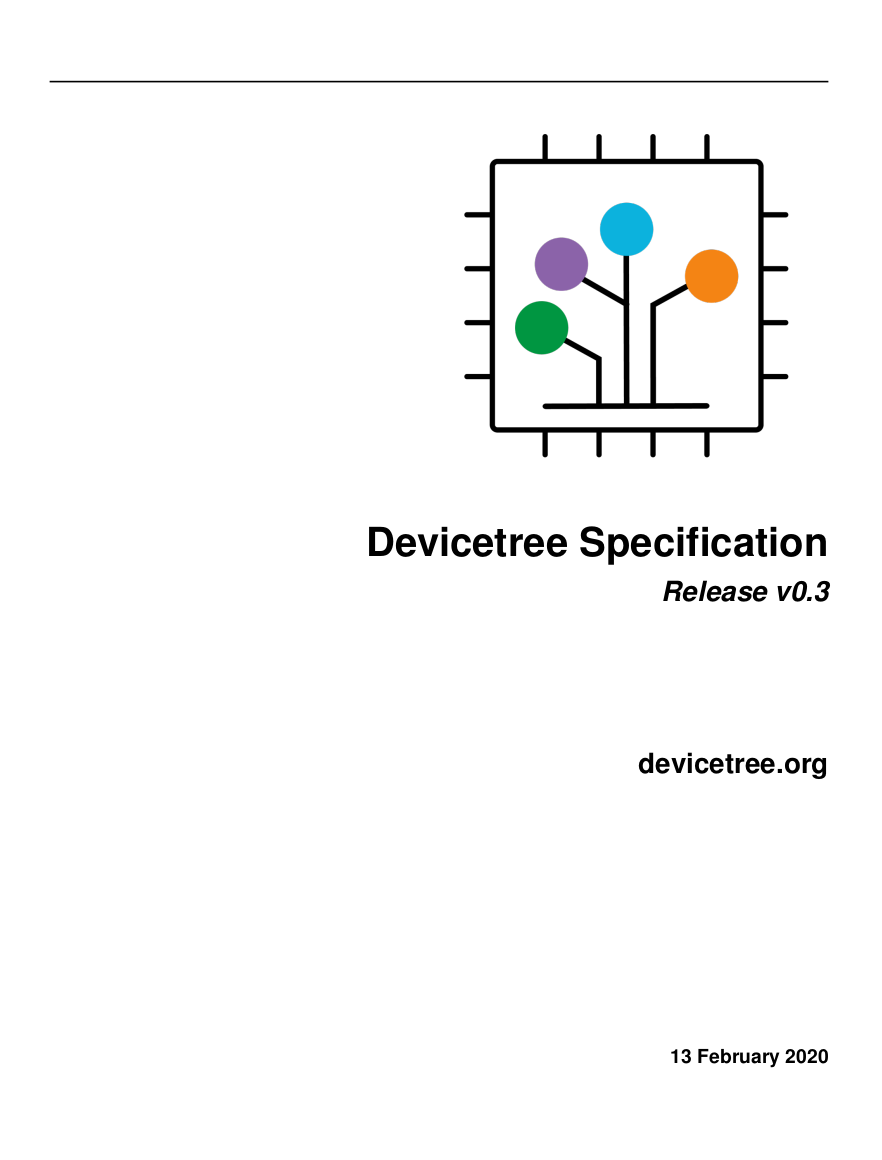
\includegraphics[width=\textwidth]{slides/sysdev-hw-devices/dt-spec.png}
  \end{columns}
\end{frame}

\begin{frame}[fragile]{Device Tree binding: legacy style}
  \begin{center}
    \kfile{Documentation/devicetree/bindings/i2c/i2c-omap.txt}
  \end{center}
  \begin{columns}[t]
    \column{0.5\textwidth}
    \begin{block}{}
      {\fontsize{5}{6}\selectfont
\begin{verbatim}
I2C for OMAP platforms

-Required properties :
- compatible : Must be
       "ti,omap2420-i2c" for OMAP2420 SoCs
       "ti,omap2430-i2c" for OMAP2430 SoCs
       "ti,omap3-i2c" for OMAP3 SoCs
       "ti,omap4-i2c" for OMAP4+ SoCs
       "ti,am654-i2c", "ti,omap4-i2c" for AM654 SoCs
       "ti,j721e-i2c", "ti,omap4-i2c" for J721E SoCs
       "ti,am64-i2c", "ti,omap4-i2c" for AM64 SoCs
- ti,hwmods : Must be "i2c<n>", n being the instance number (1-based)
- #address-cells = <1>;
- #size-cells = <0>;

Recommended properties :
- clock-frequency : Desired I2C bus clock frequency in Hz. Otherwise
  the default 100 kHz frequency will be used.

Optional properties:
- Child nodes conforming to i2c bus binding

Note: Current implementation will fetch base address, irq and dma
from omap hwmod data base during device registration.
Future plan is to migrate hwmod data base contents into device tree
blob so that, all the required data will be used from device tree dts
file.
\end{verbatim}
      }
    \end{block}
    \column{0.5\textwidth}
    \begin{block}{}
      {\fontsize{4}{5}\selectfont
\begin{verbatim}
Examples :

i2c1: i2c@0 {
    compatible = "ti,omap3-i2c";
    #address-cells = <1>;
    #size-cells = <0>;
    ti,hwmods = "i2c1";
    clock-frequency = <400000>;
};
\end{verbatim}
      }
    \end{block}
  \end{columns}

\end{frame}

\begin{frame}[fragile]{Device Tree binding: YAML style}
  \kfile{Documentation/devicetree/bindings/i2c/ti,imap4-i2c.yaml}
  \begin{columns}[t]
    \column{0.33\textwidth}
    \begin{block}{}
      {\fontsize{5}{6}\selectfont
\begin{minted}{yaml}
# SPDX-License-Identifier: (GPL-2.0-only OR BSD-2-Clause)
%YAML 1.2
---
$id: http://devicetree.org/schemas/i2c/ti,omap4-i2c.yaml#
$schema: http://devicetree.org/meta-schemas/core.yaml#

title: I2C controllers on TI's OMAP and K3 SoCs

maintainers:
  - Vignesh Raghavendra <vigneshr@ti.com>

properties:
  compatible:
    oneOf:
      - enum:
          - ti,omap2420-i2c
          - ti,omap2430-i2c
          - ti,omap3-i2c
          - ti,omap4-i2c
      - items:
          - enum:
              - ti,am4372-i2c
              - ti,am64-i2c
              - ti,am654-i2c
              - ti,j721e-i2c
          - const: ti,omap4-i2c

  reg:
    maxItems: 1
\end{minted}
      }
    \end{block}
    \column{0.33\textwidth}
    \begin{block}{}
      {\fontsize{5}{6}\selectfont
\begin{minted}{yaml}
  interrupts:
    maxItems: 1

  clocks:
    maxItems: 1

  clock-names:
    const: fck

  clock-frequency: true

  power-domains: true

  "#address-cells":
    const: 1

  "#size-cells":
    const: 0

  ti,hwmods:
    description:
      Must be "i2c<n>", n being [...]
    $ref: /schemas/types.yaml#/definitions/string
    deprecated: true

required:
  - compatible
  - reg
  - interrupts
\end{minted}
      }
    \end{block}
    \column{0.33\textwidth}
    \begin{block}{}
      {\fontsize{5}{6}\selectfont
\begin{minted}{yaml}
additionalProperties: false

if:
  properties:
    compatible:
      enum:
        - ti,omap2420-i2c
        - ti,omap2430-i2c
        - ti,omap3-i2c
        - ti,omap4-i2c
then:
  properties:
    ti,hwmods:
      items:
        - pattern: "^i2c([1-9])$"
else:
  properties:
    ti,hwmods: false

examples:
  - |
    #include <dt-bindings/interrupt-controller/irq.h>
    #include <dt-bindings/interrupt-controller/arm-gic.h>

    main_i2c0: i2c@2000000 {
        compatible = "ti,j721e-i2c", "ti,omap4-i2c";
        reg = <0x2000000 0x100>;
        interrupts = <GIC_SPI 200 IRQ_TYPE_LEVEL_HIGH>;
    };
\end{minted}
      }
    \end{block}
  \end{columns}
\end{frame}

\begin{frame}{Validating Device Tree in Linux}
  \begin{itemize}
  \item \code{dtc} only does syntactic validation
  \item YAML bindings allow to do semantic validation
  \item Linux kernel \code{make} rules:
    \begin{itemize}
    \item \code{make dt_binding_check}\\
      verify that YAML bindings are valid
    \item \code{make dtbs_check}\\
      validate DTs currently enabled against YAML bindings
    \item \code{make DT_SCHEMA_FILES=Documentation/devicetree/bindings/trivial-devices.yaml dtbs_check}\\
      validate DTs against a specific YAML binding
    \end{itemize}
  \end{itemize}
\end{frame}

\begin{frame}{The {\tt compatible} property}
  \begin{itemize}
  \item Is a list of strings
    \begin{itemize}
    \item From the most specific to the less specific
    \end{itemize}
  \item Describes the specific {\bf binding} to which the node complies.
  \item It uniquely identifies the {\bf programming model} of the
    device.
  \item Practically speaking, it is used by the operating system to
    find the {\bf appropriate driver} for this device.
  \item When describing real hardware, the typical form is
    \code{vendor,model}
  \item Examples:
    \begin{itemize}
    \item \code{compatible = "arm,armv7-timer";}
    \item \code{compatible = "st,stm32mp1-dwmac", "snps,dwmac-4.20a";}
    \item \code{compatible = "regulator-fixed";}
    \item \code{compatible = "gpio-keys";}
    \end{itemize}
  \item Special value: \code{simple-bus} $\rightarrow$ bus where all
    sub-nodes are memory-mapped devices
  \end{itemize}
\end{frame}

\begin{frame}{{\tt compatible} property and Linux kernel drivers}
  \begin{columns}
    \column{0.6\textwidth}
    \begin{itemize}
    \item Top-level DT nodes with a \code{compatible} property and
      nodes that are sub-nodes of \code{simple-bus} will cause Linux
      to identify those devices as {\bf platform devices}
      \begin{itemize}
      \item Instantiated automatically at boot time
      \end{itemize}
    \item Sub-nodes of I2C controllers $\rightarrow$ {\em I2C devices}
    \item Sub-nodes of SPI controllers $\rightarrow$ {\em SPI devices}
    \item Each Linux driver has a table of compatible strings it supports
      \begin{itemize}
      \item \kstruct{of_device_id}\code{[]}
      \end{itemize}
    \item When a DT node compatible string matches a given driver, the
      device is {\em bound} to that driver.
    \end{itemize}
    \column{0.4\textwidth}
    \includegraphics[width=\textwidth]{slides/sysdev-hw-devices/dt-to-devices.pdf}
  \end{columns}
\end{frame}

\begin{frame}[fragile]{Matching with drivers in Linux: platform driver}
  \begin{block}{\kfile{drivers/i2c/busses/i2c-omap.c}}
    {\tiny
\begin{minted}{c}
static const struct of_device_id omap_i2c_of_match[] = {
        {
                .compatible = "ti,omap4-i2c",
                .data = &omap4_pdata,
        },
        {
                .compatible = "ti,omap3-i2c",
                .data = &omap3_pdata,
        },
        [...]
        { },
};
MODULE_DEVICE_TABLE(of, omap_i2c_of_match);

[...]

static struct platform_driver omap_i2c_driver = {
        .probe          = omap_i2c_probe,
        .remove         = omap_i2c_remove,
        .driver         = {
                .name   = "omap_i2c",
                .pm     = &omap_i2c_pm_ops,
                .of_match_table = of_match_ptr(omap_i2c_of_match),
        },
};
\end{minted}
    }
  \end{block}
\end{frame}

\begin{frame}[fragile]{Matching with drivers in Linux: I2C driver}
  \begin{block}{\kfile{sound/soc/codecs/cs42l51.c}}
    {\tiny
\begin{minted}{c}
const struct of_device_id cs42l51_of_match[] = {
        { .compatible = "cirrus,cs42l51", },
        { }
};
MODULE_DEVICE_TABLE(of, cs42l51_of_match);
\end{minted}
    }
  \end{block}
  \begin{block}{\kfile{sound/soc/codecs/cs42l51-i2c.c}}
    {\tiny
\begin{minted}{c}
static struct i2c_driver cs42l51_i2c_driver = {
        .driver = {
                .name = "cs42l51",
                .of_match_table = cs42l51_of_match,
                .pm = &cs42l51_pm_ops,
        },
        .probe = cs42l51_i2c_probe,
        .remove = cs42l51_i2c_remove,
        .id_table = cs42l51_i2c_id,
};
\end{minted}
    }
  \end{block}
\end{frame}

\begin{frame}[fragile]{{\tt reg} property}
  \begin{itemize}
  \item Most important property after \code{compatible}
  \item {\bf Memory-mapped} devices: base physical address and size of
    the memory-mapped registers. Can have several entries for multiple
    register areas.
\begin{onlyenv}<1>
\begin{block}{}
\begin{verbatim}
sai4: sai@50027000 {
    reg = <0x50027000 0x4>, <0x500273f0 0x10>;
};
\end{verbatim}
\end{block}
\end{onlyenv}
\pause
  \item {\bf I2C} devices: address of the device on the I2C bus.
\begin{onlyenv}<2>
\begin{block}{}
\begin{verbatim}
&i2c1 {
   hdmi-transmitter@39 {
      reg = <0x39>;
   };
   cs42l51: cs42l51@4a {
      reg = <0x4a>;
   };
};
\end{verbatim}
\end{block}
\end{onlyenv}
\pause
  \item {\bf SPI} devices: chip select number
\begin{onlyenv}<3>
\begin{block}{}
\begin{verbatim}
&qspi {
        flash0: mx66l51235l@0 {
                reg = <0>;
        };
        flash1: mx66l51235l@1 {
                reg = <1>;
        };
};
\end{verbatim}
\end{block}
\end{onlyenv}
\pause
\item The unit address must be the address of the first \code{reg}
  entry.
\begin{onlyenv}<4>
\begin{block}{}
\begin{verbatim}
sai4: sai@50027000 {
    reg = <0x50027000 0x4>, <0x500273f0 0x10>;
};
\end{verbatim}
\end{block}
\end{onlyenv}
  \end{itemize}
\end{frame}

\begin{frame}{Status property}
  \begin{itemize}
  \item The \code{status} property indicates if the device is really in
    use or not
    \begin{itemize}
    \item \code{okay} or \code{ok} $\rightarrow$ the device is really
      in use
    \item any other value, by convention \code{disabled} $\rightarrow$
      the device is not in use
    \end{itemize}
  \item In Linux, controls if a device is instantiated
  \item In \code{.dtsi} files describing SoCs: all devices that
    interface to the outside world have \code{status = disabled}
  \item Enabled on a per-device basis in the board \code{.dts}
  \end{itemize}
\end{frame}

\begin{frame}[fragile]{Resources: interrupts, clocks, DMA, reset lines, ...}
  \begin{columns}
  \column{0.5\textwidth}
  \begin{itemize}
  \item Common pattern for resources shared by multiple hardware
    blocks
    \begin{itemize}
    \item Interrupt lines
    \item Clock controllers
    \item DMA controllers
    \item Reset controllers
    \item ...
    \end{itemize}
  \item A Device Tree node describing the {\em controller} as a device
  \item References from other nodes that use resources provided by
    this {\em controller}
  \end{itemize}
  \column{0.5\textwidth}
\begin{block}{}
{\tiny
\begin{minted}{perl}
intc: interrupt-controller@a0021000 {
   compatible = "arm,cortex-a7-gic";
   #interrupt-cells = <3>;
   interrupt-controller;
   reg = <0xa0021000 0x1000>, <0xa0022000 0x2000>;
};

rcc: rcc@50000000 {
   compatible = "st,stm32mp1-rcc", "syscon";
   reg = <0x50000000 0x1000>;
   #clock-cells = <1>;
   #reset-cells = <1>;
};

dmamux1: dma-router@48002000 {
   compatible = "st,stm32h7-dmamux";
   reg = <0x48002000 0x1c>;
   #dma-cells = <3>;
   clocks = <&rcc DMAMUX>;
   resets = <&rcc DMAMUX_R>;
};

spi3: spi@4000c000 {
   interrupts = <GIC_SPI 51 IRQ_TYPE_LEVEL_HIGH>;
   clocks = <&rcc SPI3_K>;
   resets = <&rcc SPI3_R>;
   dmas = <&dmamux1 61 0x400 0x05>,  <&dmamux1 62 0x400 0x05>;
};
\end{minted}
}
\end{block}
\end{columns}
\end{frame}

% \begin{frame}{Pin-muxing description}
%   \begin{columns}
%     \column{0.5\textwidth}
%     \begin{itemize}
%     \item Most modern SoCs, including the STM32MP1, have more features
%       than they have pins to expose those features to the outside world.
%     \item Pins are muxed: a given pin can be used for one function
%       {\bf or} another
%     \item A specific IP block in the SoC controls the muxing of pins:
%       the {\bf pinmux controller}
%     \item The Device Tree describes which pin configurations are
%       possible, and which configurations are used by the different
%       devices.
%     \end{itemize}
%     \column{0.5\textwidth}
%     \includegraphics[width=\textwidth]{slides/sysdev-hw-devices/pin-muxing-principle.pdf}
%   \end{columns}
% \end{frame}

% \begin{frame}[fragile]{Pin-muxing controllers on STM32MP1}
%   \begin{block}{\kfile{arch/arm/boot/dts/stm32mp151.dtsi}}
% {\tiny
% \begin{minted}{perl}
% pinctrl: pin-controller@50002000 {
%         #address-cells = <1>;
%         #size-cells = <1>;
%         compatible = "st,stm32mp157-pinctrl";
%         ...
%         gpioa: gpio@50002000 { ... };
%         gpiob: gpio@50003000 { ... };
%         gpioc: gpio@50004000 { ... };
%         gpiod: gpio@50005000 { ... };
%         gpioe: gpio@50006000 { ... };
%         gpiof: gpio@50007000 { ... };
%         ...
% };

% pinctrl_z: pin-controller-z@54004000 {
%         #address-cells = <1>;
%         #size-cells = <1>;
%         compatible = "st,stm32mp157-z-pinctrl";
%         ranges = <0 0x54004000 0x400>;
%         ...
%         gpioz: gpio@54004000 { .... };
%         ...
% };
% \end{minted}
% }
%   \end{block}
% \end{frame}

% \begin{frame}[fragile]{Pin-muxing configuration}
% \begin{onlyenv}<1>
%   \begin{block}{\kfile{arch/arm/boot/dts/stm32mp15-pinctrl.dtsi}}
% {\tiny
% \begin{minted}{perl}
% &pinctrl {
%         ...
%         i2c1_pins_a: i2c1-0 {
%                 pins {
%                         pinmux = <STM32_PINMUX('D', 12, AF5)>, /* I2C1_SCL */
%                                  <STM32_PINMUX('F', 15, AF5)>; /* I2C1_SDA */
%                         bias-disable;
%                         drive-open-drain;
%                         slew-rate = <0>;
%                 };
%         };
%         ...
%         m_can1_pins_a: m-can1-0 {
%                 pins1 {
%                         pinmux = <STM32_PINMUX('H', 13, AF9)>; /* CAN1_TX */
%                         slew-rate = <1>;
%                         drive-push-pull;
%                         bias-disable;
%                 };
%                 pins2 {
%                         pinmux = <STM32_PINMUX('I', 9, AF9)>; /* CAN1_RX */
%                         bias-disable;
%                 };
%         };
%         ...
% };
% \end{minted}
% }
%   \end{block}
% \end{onlyenv}
% \begin{onlyenv}<2>
%   \begin{center}
%     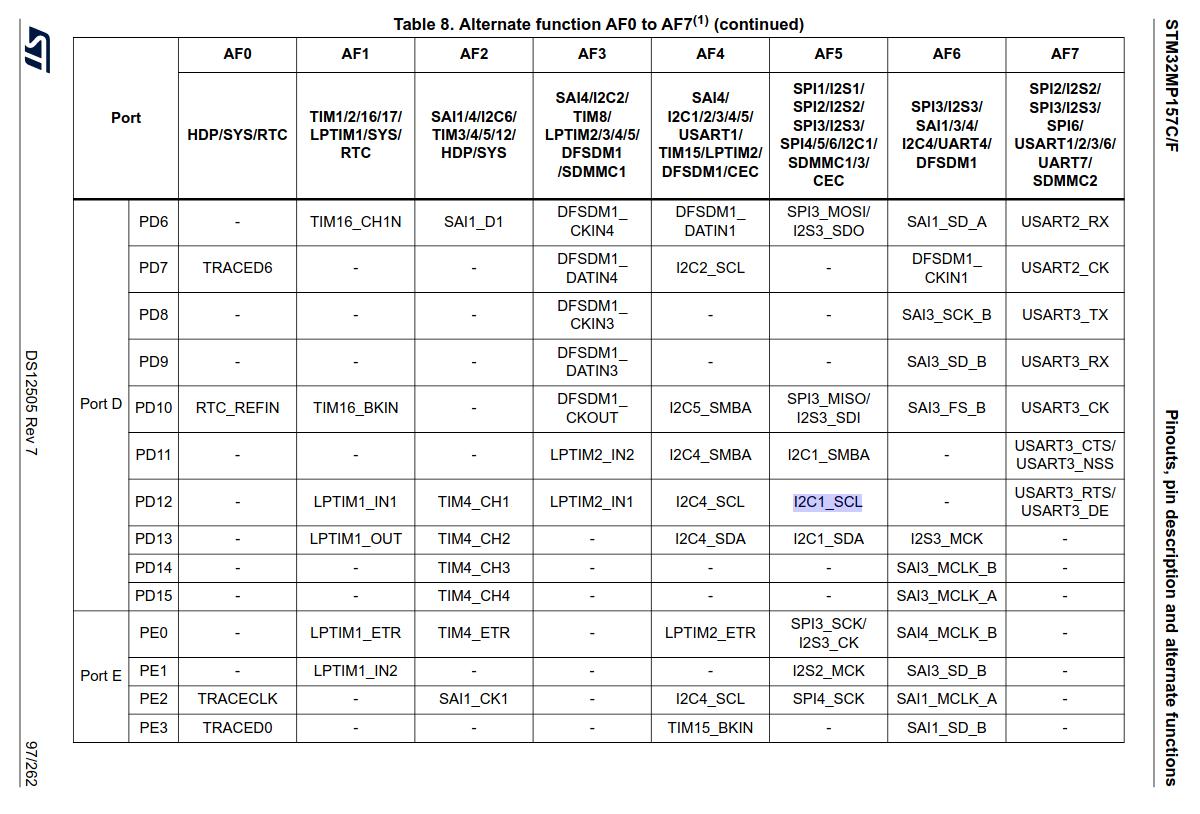
\includegraphics[height=0.78\textheight]{slides/sysdev-hw-devices/stm32mp157-i2c-pin-mux.png}
%   \end{center}
%   \tiny
%   Source: \href{https://www.st.com/resource/en/datasheet/stm32mp157c.pdf}{STM32MP157C
%   datasheet}. Note that \code{I2C1_SDA} is also available on pin \code{PF15} (not shown here).
% \end{onlyenv}
% \end{frame}

% \begin{frame}[fragile]{Pin-muxing consumer}
%   \begin{block}{}
% {\tiny
% \begin{minted}{perl}
% &i2c1 {
%         pinctrl-names = "default", "sleep";
%         pinctrl-0 = <&i2c1_pins_a>;
%         pinctrl-1 = <&i2c1_sleep_pins_a>;
%         ...
% };
% \end{minted}
% }
% \end{block}
% \begin{itemize}
% \item Typically board-specific, in \code{.dts}
% \item \code{pinctrl-0}, \code{pinctrl-1}, \code{pinctrl-X} provides
%   the pin mux configurations for the different {\bf states}
% \item \code{pinctrl-names} gives a name to each state, mandatory even
%   if only one state
% \item States are mutually exclusive
% \item The driver is responsible for switching between states
% \item \code{default} state is automatically set up when the device is
%   {\em probed}
% \end{itemize}
% \end{frame}

% \begin{frame}[fragile]{Example: LED and I2C device}
%   \begin{itemize}
%   \item Let's see how to describe an LED and an I2C device connected
%     to the DK1 platform.
%   \item Create \code{arch/arm/boot/dts/stm32mp157a-dk1-custom.dts}
%     which includes \code{stm32mp157a-dk1.dts}
%     \begin{block}{}
% {\tiny
% \begin{verbatim}
% #include "stm32mp157a-dk1.dts"
% \end{verbatim}
% }
%     \end{block}
%   \item Make sure \code{stm32mp157a-dk1-custom.dts} gets compiled to a
%     DTB by changing \kfile{arch/arm/boot/dts/Makefile}
%     \begin{block}{}
%       {\tiny
% \begin{verbatim}
% dtb-$(CONFIG_ARCH_STM32) += \
%         ...
%         stm32mp157a-dk1.dtb \
%         stm32mp157a-dk1-custom.dtb \
% \end{verbatim}
%       }
%     \end{block}
%   \item \code{make dtbs}
%     \begin{block}{}
%       {\tiny
% \begin{verbatim}
%   DTC     arch/arm/boot/dts/stm32mp157a-dk1-custom.dtb
% \end{verbatim}
%       }
%     \end{block}
%   \end{itemize}
% \end{frame}

% \begin{frame}[fragile]{Example: describe an LED}
%   \begin{columns}
%     \column{0.5\textwidth}
%   \begin{block}{stm32mp157a-dk1-custom.dts}
%     {\tiny
% \begin{minted}{perl}
% #include "stm32mp157a-dk1.dts"

% / {
%         leds {
%                 compatible = "gpio-leds";
%                 webinar {
%                         label = "webinar";
%                         gpios = <&gpioe 1 GPIO_ACTIVE_HIGH>;
%                 };
%         };
% };
% \end{minted}
%       }
%   \end{block}
%   \begin{block}{shell}
% {\tiny
% \begin{verbatim}
% # echo 255 > /sys/class/leds/webinar/brightness
% \end{verbatim}
% }
% \end{block}
%   \column{0.5\textwidth}
%   \begin{center}
%     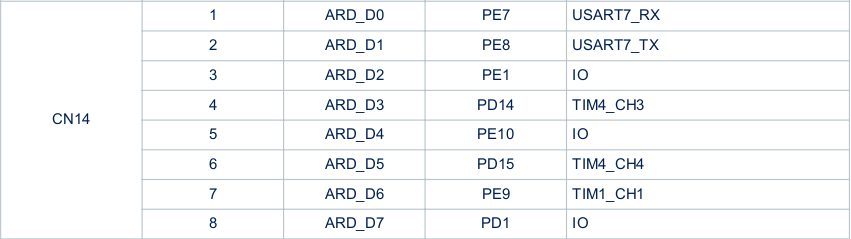
\includegraphics[height=0.3\textheight]{slides/sysdev-hw-devices/cn14-pinout.png}\\
%     \vspace{0.5cm}
%     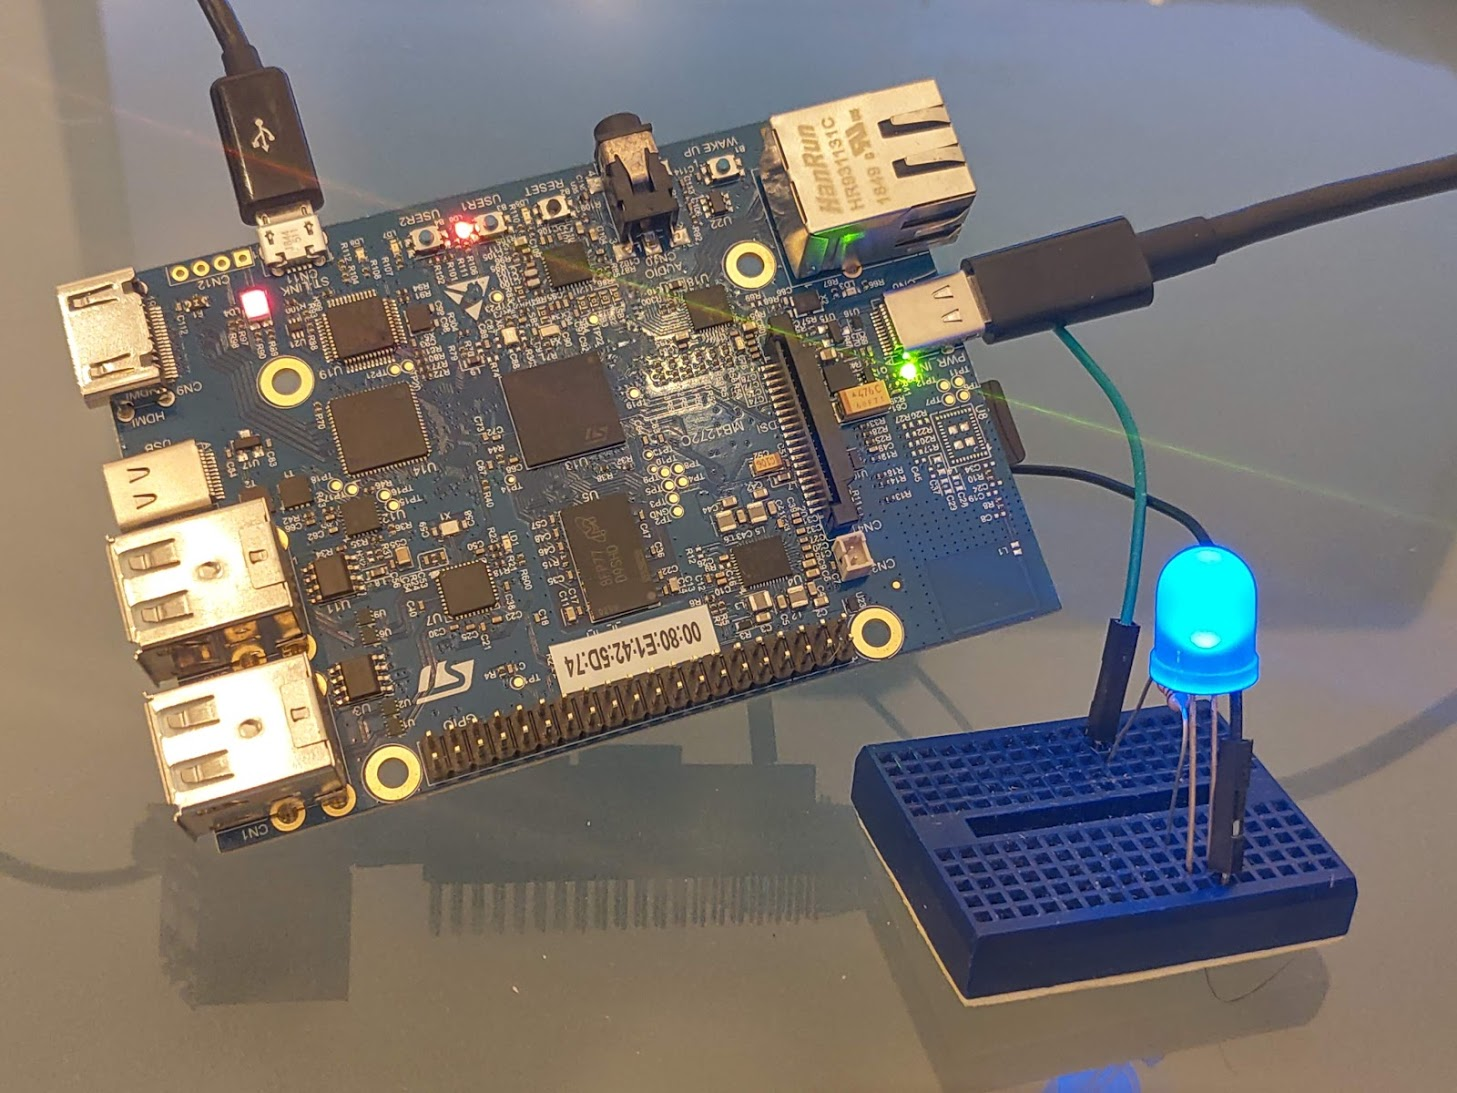
\includegraphics[height=0.3\textheight]{slides/sysdev-hw-devices/led-on.jpg}
%   \end{center}
%   \end{columns}
% \end{frame}

% \begin{frame}[fragile]{Example: connect I2C temperature, humidity and pressure sensor}
%   \begin{columns}
%     \column{0.5\textwidth}
%     \begin{block}{stm32mp157a-dk1-custom.dts}
%       {\tiny
% \begin{minted}{perl}
% &i2c5 {
%         status = "okay";
%         clock-frequency = <100000>;
%         pinctrl-names = "default", "sleep";
%         pinctrl-0 = <&i2c5_pins_a>;
%         pinctrl-1 = <&i2c5_pins_sleep_a>;

%         pressure@76 {
%                 compatible = "bosch,bme280";
%                 reg = <0x76>;
%         };
% };
% \end{minted}
% }
%   \end{block}

% \begin{block}{shell}
% {\tiny
% \begin{verbatim}
% # cat /sys/bus/iio/devices/iio\:device2/in_humidityrelative_input
% 49147
% # cat /sys/bus/iio/devices/iio\:device2/in_pressure_input
% 101.567167968
% # cat /sys/bus/iio/devices/iio\:device2/in_temp_input
% 24380
% \end{verbatim}
% }
% \end{block}
%   \column{0.5\textwidth}
%   \begin{center}
%     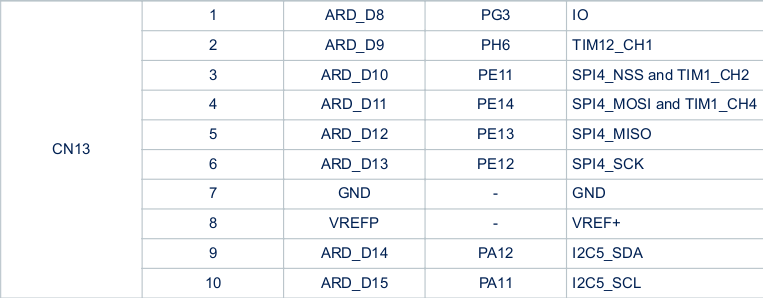
\includegraphics[width=\textwidth]{slides/sysdev-hw-devices/cn13-pinout.png}\\
%     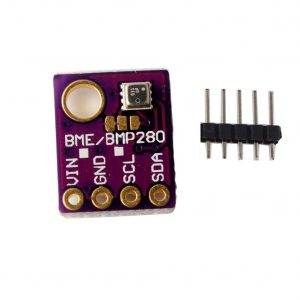
\includegraphics[width=0.4\textwidth]{slides/sysdev-hw-devices/bme.jpg}
%   \end{center}
% \end{columns}
% \vspace{0.5cm}
% Details at
% \url{https://bootlin.com/blog/building-a-linux-system-for-the-stm32mp1-connecting-an-i2c-sensor/}

% \end{frame}

\begin{frame}
  \frametitle{References}
  \begin{columns}
    \column{0.6\textwidth}
       \begin{itemize}
       \item Device Tree 101 webinar, Thomas Petazzoni (2021):\\
	     Slides: \url{https://bootlin.com/blog/device-tree-101-webinar-slides-and-videos/}\\
	     Video: \url{https://youtu.be/a9CZ1Uk3OYQ}
       \item Kernel documentation
         \begin{itemize}
         \item \kdochtmldir{driver-api/driver-model}
         \item \kdochtmldir{devicetree}
         \item \kdochtml{filesystems/sysfs}
         \end{itemize}
      \item \url{https://devicetree.org}
       \item The kernel source code
         \begin{itemize}
         \item Full of examples of other drivers!
         \end{itemize}
       \end{itemize}
    \column{0.4\textwidth}
    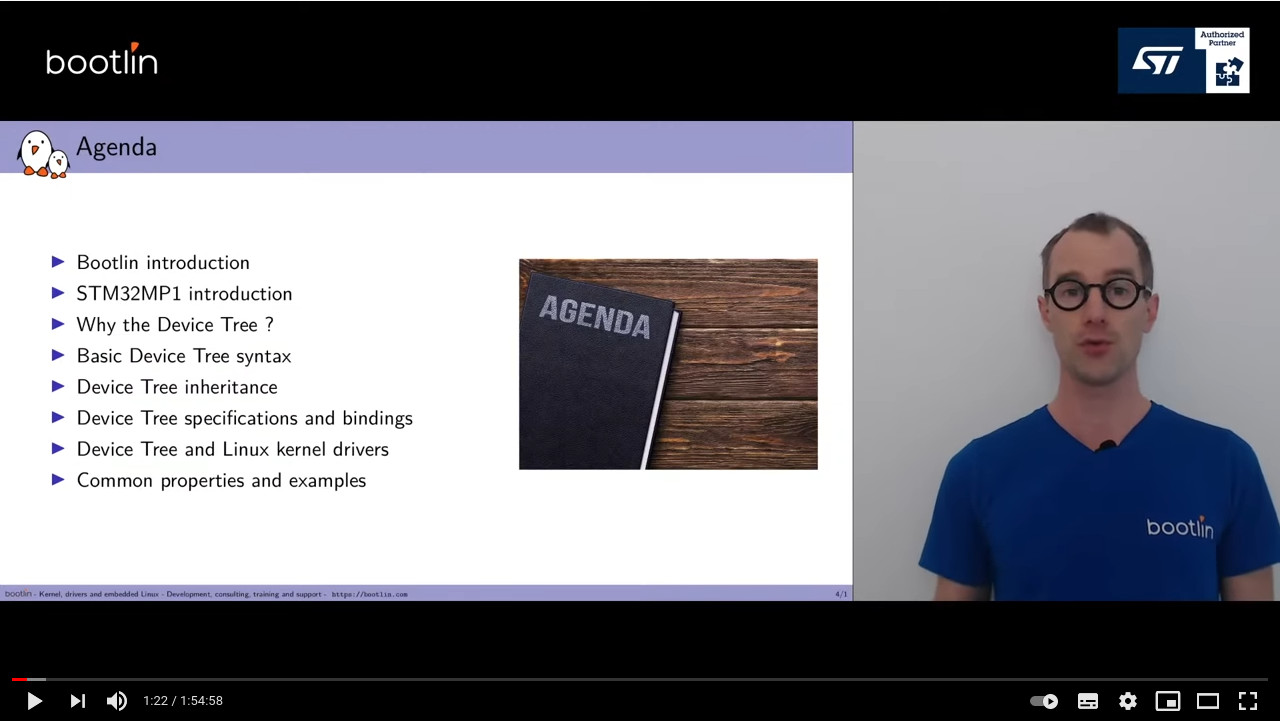
\includegraphics[width=\textwidth]{common/device-tree-video.jpg}
  \end{columns}
\end{frame}

\subsection{Discoverable hardware: USB and PCI}

\begin{frame}{Discoverable hardware}
  \begin{itemize}
  \item Some busses have built-in hardware discoverability mechanisms
  \item Most common busses: USB and PCI
  \item Hardware devices can be enumerated, and their characteristics
    retrieved with just a driver or the bus controller
  \item Useful Linux commands
    \begin{itemize}
    \item \code{lsusb}, lists all USB devices detected
    \item \code{lspci}, lists all PCI devices detected
    \item A detected device does not mean it has a kernel driver
      associated to it!
    \end{itemize}
  \item Association with kernel drivers done based on product
    ID/vendor ID, or some other characteristics of the device: device
    class, device sub-class, etc.
  \end{itemize}
\end{frame}


% \setuplabframe
% {Accessing hardware devices}
% {
%   Time to start the practical lab!
%   \begin{itemize}
%   \item Exploring the contents of \code{/dev} and \code{/sys} and the
%     devices available on the embedded hardware platform.
%   \item Using GPIOs and LEDs.
%   \item Modifying the Device Tree to control pin multiplexing and
%         declare an I2C-connected joystick.
%   \item Adding support for a USB audio card using Linux kernel modules
%   \item Adding support for the I2C-connected joystick through
%         an out-of-tree module.
%   \end{itemize}
% }
